\documentclass[../main.tex]{subfiles}

\begin{document}

In this section we will prove some different properties about the modal logic
\textbf{GL}, that was introduced in chapter \ref{chap:Pre}.
These properties will be used in the following chapters. Some of these properties might
hold in other modal logics, but we will look at \GL\ as our base logic,
instead of a more common modal logic like \textbf{K}.
Further in the end we will introduce the system $\text{\textbf{GLS}}$.

This section will follow \cite{Smor1985}. But there will be a some small
differences. Smorynski calls the logic \textbf{GL} for \textbf{PRL} which
stands for \textit{Pr}ovability \textit{L}ogic, and he denotes the logic we
have called \textbf{GLS} by $\textbf{PRL}^\omega$.\footnote{He also have a
slightly different definition of a Kripke model.}

This section (and the next one) dose not use the preceding sections about recursive functions. We will only
focus on modal logic or anything about Gödel's Incompleteness Theorems. In
chapter \ref{chap:Complete} we will combine all three parts; the recursion
theory, the arithmetics and the modal logic.


Finiteness of $W$ in such a model?
\section{Tress and \GL}

It is known that \textbf{GL} is weakly complete with resect to conversely
well-founded transitive frames. There is another result that is in the same
vein; \textbf{GL} is complete with respect to finite tress. The goal of this
section is to prove this result. We will first start of by defining the notion
of a tree and a few results about these.

\subsection{Trees}
In this subsection the notion of a special type of graphs called tress will be
introduce. The goal of this section is to prove Könings lemma about trees. We
will start of by defining the notion of a tree.
\begin{defi}
	A \textit{tree} is a tuple $\mathcal{T}=\la W,R,w_0\ra$ where $(W,R)$ where:
	\begin{enumerate}
		\item $<$ is transitive and asymmetric.
		\item $w_0$ is the minimal element of $<$. I.e $w_0
			<w$ for all $w\in W$.
		\item The set of predecessors of any element is finite and
			linearly ordered by $<$.
	\end{enumerate}
	A tree is \textit{infinite} if the set $W$ is infinite.
\end{defi}

We will state some immediate definitions, that should be known from the course
\textit{Diskret matematik}:
\begin{defi}
	The \textit{nodes} of a tree $\mathcal{T}=\la W,R,w_0\ra$ are the
	elements of the set $W$.

	If $w,v\in W$ are nodes and  $wRv$ then we say that they are joined  by an \textit{edge}.


	A \textit{walk} is an altering series of vertices and edges in
	which for each $v$ we have that $wRv$ for the $w$ immediate before it 
	. We call a walk for a \textit{trail}, if all the edges in
	the walk are distinct. A \textit{path} is trail in which all the
	nodes are different.
\end{defi}


It is know from the course \textit{Diskret matematik} that between any two
vertices there are exactly one path in a tree. 
As the concept of a tree is assumed know, we will not look at any concrete
examples,
We will need
some further definitions to state and prove Könings lemma:
\begin{defi}
	Let $w\in W$. The \textit{degree} of of $w$ in $\mathcal{T}$ is the
	number of edges incident to it.
\end{defi}
\begin{defi}
	Let $w$ be a node of a tree $\mathcal{T}$, we then define the map
	$\pi:\mathcal{T}\setminus\{w_0\}\rightarrow\mathcal{T}$ in the
	following way:
	\[\pi(w)=\text{The node adjacent to}\ w\ \text{on the path to}\ w_0\]
	We call $\pi(w)$ the \textit{parent node} of $w$. 

	The \textit{child nodes} of $w$ are the elements of the set
	$\{v\mathcal{T}:\pi(v)=w\}$, i.e the child nodes of $w$ are all the
	nodes of $\mathcal{T}$ to which $w$ is the parent. If $w$ has no child
	nodes it is called a \textit{leaf node}.
\end{defi}
It is clear that if $w$ is a leaf node, then degree of $w$ is $1$.
\begin{defi}
	A subset $\Gamma$ of a tree $\mathcal{T}$ is called a
	\textit{branch} if and only if all the following conditions holds:
	\begin{enumerate}
		\item $w_0\in\Gamma$
		\item The parent node of each $w\in\Gamma\setminus\{w_0\}$ is
			in $\Gamma$
		\item Each node in $\Gamma$ is either a leaf node in
			$\mathcal{T}$ or has exactly one child node in
			$\Gamma$.
	\end{enumerate}
	A branch $\Gamma$ is called \textit{infinite} if and only if it has no
	leaf node at the end.
\end{defi}
\begin{defi}
	A \textit{fork} of a $\mathcal{T}$ is a node of $\mathcal{T}$ which is the end
	point of two or more branches.
\end{defi}
\begin{defi}
	A tree $\mathcal{T}$ is called a \textit{finitely branching tree} if
	every node of $\mathcal{T}$ has finitely many child nodes.
\end{defi}

The proof of Könings lemma will depend on the following axiom:
\begin{axiom}[Axiom of Dependent Choice]
	Let $R$ be an relation on a set $W$ and suppose that:
	\[\forall w\in W\exists v\in W: wRv\]
	Then there exists a sequence $(w_n)_{n\in\omega}\in W$ such that
	\[\forall n\in\omega: w_nRw_{n+1}\]
\end{axiom}

This axiom is a weak form of the axiom of choice, so some of the consequnces of
the axiom of choice also follows from this axiom. \textbf{Er dette overhovedt
vigtigt at kommentere på?}

In the proof of Köning's
lemma we will look at the subset of all nodes with infinitely many descendants
and the relation $R$ where we have that for nodes $w,v\in W$:  $wRv$ if and only if $v$ is a child of $w$. This relation and
set
fulfills the conditions of the axiom and we can thus create the sequence
$(w_n)_{n\in\omega}$.

We can now state Köning's lemma:
\begin{lemma}{Köning's lemma}
	\label{lem:kong}
	Let $\mathcal{T}$ be a finitely branching tree. Then it is infinite if
	and only if has an infinite path.
\end{lemma}
\begin{proof}
	If $\mathcal{T}$ has an infinite path, then it is trivial true that
	$\mathcal{T}$ is infinite. 

	For the other way, assume that $\mathcal{T}$ is infinite. To show that
	$\mathcal{T}$ has an infinite path is the same as showing that it has
	an infinite branch. We will show that there is a sequence of nodes
	$w=(w_0,w_1,w_2,\ldots)$ in $\mathcal{T}$ such that the following holds:
	\begin{enumerate}
		\item $w_0$ is the root node
		\item $w_{n+1}$ is a child node of $t_n$
		\item each $w_n$ has infinitely many descendants (definer
			dette, selvom det giver god mening).
	\end{enumerate}
	Then $w$ is a branch of infinite length, and thus $\mathcal{T}$ has an
	infinite path.

	We start with the root node $w_0$. It has a finite number of child
	nodes. Suppose for contradiction that each of these child nodes had a
	finite number of descendants, but thus would mean that $w_0$ would have
	a finite number of descendants and thus that $\mathcal{T}$ would be
	finite. Therefore $w_0$ has a child node with infinitely many
	descendants; let $w_1$ be one of those.

	Now suppose that node $w_k$ has infinitely many descendants. By the
	same argument as before we get that $w_k$ has at least one child node
	with finitely many descendants. Let $w_{k+1}$ be one of these. We have
	thus shown how the sequence $w$ can be constructed, and the lemma
	follows by the axiom of dependent choice
\end{proof}
It is clear that finite trees are conversely well-founded frames. This fact is crucial
in the proof of theorem in the next subsection, that can be seen as strengthening of the
weak completeness theorem of chapter \ref{chap:Pre}:
\subsection{The Finite Tree Theorem}
The following theorem is a strengthening of the weak completeness theorem for
\GL, since trees are a subset of the transitive conversely well-founded models
and we by this theorem get that we can with out loss of generality assume that
our model is finite. This last feature will be crucial in the proof of main
theorems of the next chapter.
\begin{thm}[The Finite Tree Theorem]
	Let $\alpha$ be a modal formula. Then the following are equivalent:
	\begin{enumerate}
		\item $\vdash_\GL\alpha$
		\item $\alpha$ is true in all models on finite trees
		\item $\alpha$ is valid in all models on finite trees
	\end{enumerate}
\end{thm}
With this theorem it is possible to only consider finite frames. This will make
the proof of our main theorem of chapter \ref{chap:Complete} possible.
\begin{proof}
	The implications $(1)\Rightarrow (2)$ and $(1)\Rightarrow(3)$ follows
	by the completeness theorem. We also have that $(2)\Leftrightarrow (3)$
	is true [Kom med et kort argument]. Thus we will just have to show $(2)\Rightarrow(1)$

	We will show this by contraposition, i.e $\neg(1)\Rightarrow\neg(2)$.
	Assume that $\not\vdash_{\GL}\alpha$ and
let $\mathcal{K}$ be the following model $\mathcal{K}=\la W,R,w_0,\phi\ra $ be a counter model i.e
	$\not\vDash_{w_0}^{K'}\alpha$. Let $S$ be the set of subformulas of
	$\alpha$ The goal is now to define a finite tree
	model: $\mathcal{K}_T=\la W_T,<_T,\phi_T\ra$. We will do this be
	letting $W_T$ consists of finite $R$-increasing sequences form $K$.

	\textbf{Stage 0:} Let the sequence $w_0$ be a part of $K_T$.

	\textbf{Stage $n+1$:} For each sequence $(w_0,\ldots w_n)\in W_T$ we
	will look at $\Gamma=\{\Box\beta\in S(\alpha):\
	w_n\in\phi(\Box\beta)\}$.
	If $\Gamma=\emptyset$ then we do not extend the sequence $(w_0,\ldots
	w_n)$. Otherwise we will for each $\Box\beta\in\Gamma$ choose a node
	$v\in W$ such that $w_0Rv$ and such that we have:
	$$v\in\phi(\Box\beta),\ v\not\in\phi(\beta)$$
	We can do this because of axiom 3. We will then add the sequence
	$(w_0,\ldots w_n,v)$ to the set $W_T$

	The model $\mathcal{K}_T$ then further consists of $<_T$ is the strict
	ordering by extension of finite sequences. $\phi_T$ is the defined in
	the following way:
	$$(w_0,\ldots,w_n)\in \phi_T(p)\Leftrightarrow w_n\in\phi(p)$$
	This leads way to the following notation that we will use in the rest
	of the proof:
	$$\vDash_{(w_0,\ldots,w_n)}^{\mathcal{K}_T}p\Leftrightarrow\vDash_{w_n}^\mathcal{K} p$$
	We will now prove two claims, by which the theorem will follow 

	\textbf{Claim 1:} $\mathcal{T}=(W_T,<_T,w_0)$ is a finite tree with origin $(w_0)$.
	Finiteness follows from lemma \ref{lem:kong}, since the $\mathcal{T}$
	is finitely branching since the branches correlated with the elements
	of $S$. Further there is no infinite paths in $\mathcal{T}$, since when
	we go from $(w_0,\ldots w_n)$ to $(w_0,\ldots, w_n,w_{n+1})$ we one
	sentence from $\Box\beta\in S$ gets forced by $w_{n+1 }$ and since
	these are finite, the process will stop at some point, and thus the
	path will be finite.

	\textbf{Claim 2:} For all $\beta\in S(\alpha)$ and for all $(w_0,\ldots
	w_n)\in W_T$ we have:
	$$\vDash^{\mathcal{K}_T}_{(w_0,\ldots,w_n)}\beta\Leftrightarrow\ \vDash_{w_n}^\mathcal{K}\beta$$
	This proof is done by induction on the complexity of $\beta$. We will
	only look at the case $\beta=\Box\gamma$. So we have by the induction
	hypothesis:
	\begin{align*}
		\vDash_{w_0}\Box\gamma&\Rightarrow\forall v(w_0Rv\Rightarrow\ 
		\vDash_v\gamma)\\
				      &\Rightarrow\forall v((w_0,\ldots
				      w_n,v)\in W_T\Rightarrow\
				      \vDash_v\gamma)\\
				      &\Rightarrow\forall v((w_0,\ldots
				      w_n,v)\in W_T\Rightarrow\
				      \vDash_{(w_0,\ldots w_n,v)}^{\mathcal{K}_T}\gamma)
	\end{align*}
	And the last line is the same as $\vDash_{(w_0,\ldots,w_n)}\Box\gamma$
	For the other way, we will use contraposition:
	\begin{align*}
		\not\vDash_{w_0}\Box\gamma&\Rightarrow \exists v(w_0Rv\ \&\
		\not\vDash_v\gamma)\\
					  &\Rightarrow\exists v((w_0,\ldots
					  w_n,v)\in W_T\ \&\
					  \not\vDash_v\gamma)\\
					  &\Rightarrow\exists v((w_0,\ldots
					  w_n,v)\in W_T\ \&\
					  \not\vDash_{(w_0,\ldots,w_n,v)}^{\mathcal{K}_T}\gamma)
	\end{align*}
	And the last line is the same as
	$\not\vDash_{(w_0,\ldots,w_n)}\Box\gamma$. 

	The theorem now follows since we have:
	$$\not\vDash_{w_0}\alpha\Rightarrow\
	\not\vDash_{[w_0)}^{\mathcal{K}_T}\alpha$$
\end{proof}

From this theorem there follows a number of interisting corrolaies:

\begin{cor}
	\GL\ is decidable.\textbf{Definer lige hvad dette betyder}
\end{cor}
\begin{cor}
	\label{cor:Nec}
	For all formulas $\alpha$ we have:
	\[\vdash_\GL\alpha\Leftrightarrow\vdash_\GL\Box\alpha\]
\end{cor}

From this theorem, we can also find the minimum element of a Kripke model of
\GL. This leads to the following definition:

\begin{defi}
	Let $\mathcal{K}=\la W,R,\phi\ra$ be a Kripke model. A \textit{pointed
	Kripke model} is a pair $\la \mathcal{K},w_0\ra$ where $w_0$ is a node
	of $W$. In the rest of this project we will have that $w_0$ is the
	minimum node of the tree of \GL. We will often just define a pointed
	Kripke as $\mathcal{K}=\la W,R,\phi,w_0\ra$.
\end{defi}

\section{The Continuity Theorem}
In this section the continuity theorem and a corollary of it will be stated and
proven. This section applies to all Kripke model, and thus is not only about
\GL.

We will first need to definitions:
\begin{defi}
	We define $d(\alpha)$ in the following way: $d(p)=d(\bot)=0$,
	$d(\alpha\rightarrow\beta)=\text{max}(d(\alpha),d(\beta))$ and
	$d(\Box(\alpha)=d(\alpha)+1$. So $d(\alpha)$ is the maximal number of
	nested occurences of $\Box$ in $\alpha$. We call $d(\alpha)$ the modal
	degree of $\alpha$.
\end{defi}

\begin{defi}
	Let $R$ be a relation on a set $W$. For each $i\in\omega$ define $R^i$
	as follows: $R^0$ is the identity relation on $W$. $R^{i+1}=\{\la
	w,v\ra: \exists v'(wR^iv'\wedge v'Rv\}$. This $R^1=R$ and $wR^nv$ if
	and only if $\exists v_0,\ldots v_n(w=v_0R\ldots Rv_n=v)$.
\end{defi}
\begin{thm}[The Continuity Theorem]
	\label{thm:conti}
	Let $\mathcal{K}=\la W,R,\phi\ra$ and $\mathcal{K}'=\la V,S,\phi'\ra$
	be models and let $w\in W$. Let $P\subseteq \Phi$ be a set of proportional letters.
	Suppose that $d(\alpha)=n$, that all proportional letters that occur in 
	$\alpha$ are in $P$, $\{v:\exists i\leq n\ wR^iv\}$, $S=\{\la
	v,v'\ra:x,y\in V\wedge vRv'\}$, and $p\in \phi'(v)$ if and only if
	$p\in\phi(v)$ for all $v\in V$ and all proportional letters in $P$. 
	Then $\vDash_w^\mathcal{K}\alpha$ if and only if
	$\vDash_w^{\mathcal{K'}}\alpha$.
\end{thm}
\begin{proof}
	We will show that for all subformulas $\beta$ of $\alpha$, if we for some
	$i$ have that $wR^iv$ and $d(\beta)+i\leq n$ such that $i\leq n$ and
	$v\in V$, then $\vDash_v^\mathcal{K}\beta$ if and only if
	$\vDash_v^{\mathcal{K}'}\beta$. Since $wR^0w$ and $d(\alpha)=0$ the
	theorem will follow.

	The proof will be induction on the complexity if $\beta$. 
	The cases where $\beta$ is $\bot$ or a $p\in P$ is trivial. If $\beta$
	is $\gamma\rightarrow\sigma$ then $d(\gamma),d(\sigma)\leq d(\beta)$
	and the result follows the induction hypothesis.
	If $\beta$ is $\box\gamma$, $WR^iv$ and $d(\beta)+i\leq n$. Then $v\in
	V$ and $d(\beta)=d(\gamma)+1$. If $vRv'$ then $wR^{i+1}v'$,
	$d(\gamma)+i+1\leq n$, $v'\in V$ and therefore $vSv'$ and by the
	induction hypothesis we get $\vDash_{v'}^\mathcal{K}\Gamma$ if and only
	if $\vDash_{v'}^{\mathcal{K}'}\gamma$, since we have that $S\subseteq
	R$, $vRv'$ if $vSv'$. But this means that $\vDash_v^\mathcal{K}\beta$ if
	and only if for all $v'$ such that $vRv'$ we have that
	$\vDash_{v'}^{\mathcal{K}'}\gamma$; if and only if for all $v'$ such
	that $vSv'$: $\vDash_{v'}^\mathcal{K}\gamma$ if and only if by the
	induction hypothesis for all $v'$ such that $vSv'$;
	$\vDash_{v'}^{\mathcal{K}'}\gamma$ if and only if
	$\vDash_v^{\mathcal{K}'}\beta$.
\end{proof}

From this theorem the following corollary is a immediate consequence and we
will use it to prove parts of the main theorem of the next chapter:
\begin{cor}\label{cor:conti}
	Let $\alpha$ be a formula. Let $\mathcal{K}=\la W,R,\phi\ra$ and
	$\mathcal{K}'=\la V,R,\phi'\ra$ be models, and $p\in\phi(w)$ if and
	only if $p\in\phi'(w)$ for all $w\in W$ and all $p$ contained in
	$\alpha$.
	Then $\vDash_w^\mathcal{K}\alpha$ if and only if
	$\vDash_w^{\mathcal{K}'}\alpha$.
\end{cor}

\section{The system \text{\textbf{GLS}}}

In this section we will define the modal logic \textbf{GLS} (The "S" is for
Solovay). Before we can do
this in a smart way, we will define the notion of a Nec free axiomation; i.e a
system that is not closed under the rule Nec. We have to do this, since the
system \GLS\ will extend \GL\ but is not closed under the rule nec.

\subsection{Avoiding Nec}

In this section we will take \textbf{K4} as our base logic and see \GL\  as an
extension of this.
We will need the following notation to
define this. Given a set $\Gamma$:
\begin{enumerate}
	\item $\Gamma\vdash_{\textbf{MP}}\alpha$ if $\alpha$ is derivable form $\Gamma$ by
		only using $R1$
	\item $\Gamma\vdash_{\textbf{Nec}}\alpha$ if $\alpha$ is derivable form $\Gamma$ by
		using $R1$ and $R2$.
\end{enumerate}
We will further define the following set for any set $\Gamma$:
\[
	\Gamma^{\textbf{Nec}}=\Gamma\cup\{\Box\beta:\beta\in\Gamma\}
\]
This set allows us to avoid Nec by the axioms of \textbf{K4}, which the
following lemma shows:
\begin{lem}
	Let $\Gamma$ include all the instances  of axioms of \textbf{K4}. Then:
	\[
		\Gamma\vdash_{\textbf{Nec}}\alpha\Leftrightarrow\Gamma^{\textbf{Nec}}\vdash_{\textbf{MP}}\alpha
	\]
\end{lem}
\begin{proof}
	The way $\Leftarrow$ is trivial. So we will only show $\Rightarrow$.
	To prove this, it is enough to show that the set of theorems of
	$\Gamma^{\textbf{Nec}}$ is closed under $R2$; i.e to show that:

\[\Gamma^{\textbf{Nec}}\vdash\alpha\Rightarrow\Gamma^{\textbf{Nec}}\vdash_{\textbf{MP}}\Box\alpha\]

Let $\Gamma^{\textbf{Nec}}\vdash_{\textbf{MP}}\alpha$. Then we have a sequence
	$\alpha_1,\ldots,\alpha_n=\alpha$, where for each $1\leq i\leq n$ we
	have that $\alpha_i$ is one of the following three:
	\begin{enumerate}
		\item We have that it is an axiom $\alpha_i\in\Gamma$ 
		\item It is the necessitation  $\Box\beta_1$ of an axiom
			$\beta_1\in\Gamma$
		\item It is a consequence of \textbf{MP} of
			$\alpha_j,\alpha_k=\alpha_j\rightarrow\alpha_i$
			where $j,k<i$.
	\end{enumerate}
	We will show  by induction on the length $i$ of a 'initial' segment
	$\alpha_1,\ldots,\alpha_i$ that
	$\Gamma^{\textbf{Nec}}\vdash_{\textbf{MP}}\Box\alpha_i$. 
	\begin{enumerate}
		\item If we have that $\alpha_i\in\Gamma$. Then by definition
			we have that $\Box\alpha_i\in\Gamma^{\textbf{Nec}}$ and thus
			$\Gamma^{\textbf{Nec}}\vdash_{\textbf{MP}}\Box\alpha_i$.
		\item If $\alpha_i=\Box\beta_i$ for some $\beta_i\in\Gamma$,
			then we can make the following deduction:
			\begin{align*}
				\Gamma^{\textbf{Nec}}&\vdash_{\textbf{MP}}\Box\beta_i &\text{Since}\
				\Box\beta_i\in\Gamma^{\textbf{Nec}}\\
						     &\vdash_{\textbf{NP}}\Box\beta_i\rightarrow\Box\Box\beta_i
					&\text{By}\ \textbf{4}\\
					&\vdash_{\textbf{MP}}\Box\Box\beta_i\ (=\Box\alpha_i) 
					&\text{By}\ \textbf{MP}
			\end{align*}
			Which shows the result.
		\item If $\alpha_i$ follows form
			$\alpha_j,\alpha_k=\alpha_j\rightarrow\alpha_i$ by
			\textbf{MP} we have by the induction hypothesis that
			$\Gamma^{\textbf{Nec}}\vdash_{\textbf{MP}}\Box\alpha_j$ and
			$\Gamma^{\textbf{Nec}}\vdash_{\textbf{MP}}\Box(\alpha_j\rightarrow\alpha_i)$. By
			\textbf{K} we also have that
			$\Gamma^2\vdash_{\textbf{MP}}\Box\alpha_j\wedge\Box(\alpha_j\rightarrow\alpha_i)\rightarrow\Box\alpha_i$
			and by propositional logic we get that:
			$\Gamma^2\vdash_{\textbf{MP}}\Box\alpha_i$.
	\end{enumerate}
	This ends the induction and the lemma will follow.
\end{proof}
By this lemma we can get a \textbf{Nec}-free definition of \textbf{K4} and \GL\  that we will call
$\textbf{K4}^{\textbf{Nec}}$ and $\GL^{\textbf{Nec}}$. We can further by the deduction theorem from propositional logic get
the following:

\begin{lem}
	$\Gamma\vdash\alpha$ iff there is a finite set
$\{\gamma_0,\ldots,\gamma_{n-1}\}\subseteq \Gamma$ such that:
$K\vdash\wedge\gamma_i\rightarrow\alpha$
\end{lem}

\subsection{Definition of \textbf{GLS}}
\begin{defi}
	The system of modal logic \text{\textbf{GLS}} is defined as the system
	of propositional modal logic that have all the theorems of
	$\GL^{\textbf{Nec}}$\ and
	 addition of the axiom of Reflexion: 
	 \begin{enumerate}
		 \item[\textit{Refl}:]$\Box\alpha\rightarrow\alpha$ 
 	\end{enumerate}
	and which sole rule of inference is \textit{modus ponens}. 
\end{defi}
It should be noted that this modal logic is not a \textit{normal} one.
The main theorem about this modal logic is the following, which gives a sort of
model theory for \GLS.
\begin{thm}
	\label{thm:MainGLS}
	Let $\alpha$ be a modal formulas. Define the following set: $S_\Box(\alpha)=\{\Box\beta:\
	\Box\beta\ \text{ is a subformula of}\ \alpha\}$ the set of
	subformulas of $\alpha$ that is boxed. Then the following to
	statements are equivalent:
	\begin{enumerate}
		\item $\vdash_\GLS\alpha$
		\item $\vdash_\GL\bigwedge_{\Box\beta\in
			S_\Box(\alpha)}(\Box\beta\rightarrow\beta)\rightarrow\alpha$
	\end{enumerate}
\end{thm}

This theorem reduces the decidability of \GLS to the decidability of \GL and
describes a model theory for \GLS.

\begin{defi}
	A model $\mathcal{K}=\la W,R,\phi\ra$ with start node $w_0$ is $\alpha$-sound if for every
	$\Box\beta\in S_\Box(\alpha)$  we have:
	$\vDash_{w_0}\Box\beta\rightarrow\beta$
\end{defi}
We can reduce theorem \ref{thm:MainGLS} to the following:
\begin{thm}
	\label{thm:lll}
	Let $\alpha$ be a modal formulas. Then:
	\begin{enumerate}
		\item $\vdash_\GLS\alpha$ iff $\alpha$ is true in all
			$\alpha$-sound models of $\GL$
		\item $\vdash_\GL\alpha$ iff $\alpha$ is valid in all
			$\alpha$-sound models of $\GL$
	\end{enumerate}
\end{thm}
\begin{proof}[Proof that \ref{thm:lll}\ \Rightarrow\ \ref{thm:MainGLS}:]
	Assume \ref{thm:lll}.1. We hen have that $\vdash_\GLS\alpha$ iff $\alpha$ is true in all
	$\alpha$-sound models of $\GL$; which is the same all models of
	$\GL+\bigwedge_{\Box\beta\in S_\Box(\alpha)}(\Box\beta\rightarrow\beta)=\GL^s$ and hence:
	$$\vdash_\GLS\alpha\Leftrightarrow\vdash_{\GL^s}\alpha$$
\end{proof}
From theorem \ref{thm:lll} we get the following corollary:
\begin{cor}
	Let $\alpha$ be a modal formula. Then:
	\[\vdash_\GL\alpha \Leftrightarrow\ \vdash_\GLS\Box\alpha\]
\end{cor}
\begin{proof}
	"$\textbf{"\Rightarrow":}$ We have that
	\begin{align*}
		\vdash_\GL\alpha &\Rightarrow\vdash_\GL\Box\alpha, \ \text{By
		closure under nec}\\
				 &\Rightarrow \vdash_\GLS\Box\alpha 
	\end{align*}

	"$\textbf{"\Leftarrow":}$ We see that we have
	\begin{align*}
		\vdash_\GLS\Box\alpha\ &\Rightarrow\ \Box\alpha\ \text{is true
		in all}\ \Box\alpha\text{-sound model of}\ \GL\\
				       &\Rightarrow\ \vdash_\GL\Box\alpha\\
				       &\Rightarrow\ \vdash_\GL\alpha
	\end{align*}
	Where the last deduction follows form corollary \ref{cor:Nec}.
\end{proof}
For the proof of \ref{thm:lll} we will make use of the following usefull
construction:

\begin{defi}
	Let $\mathcal{K}=\la W,R,\phi\ra$ be a Kripke Model. The derived model
	$\mathcal{K'}$ is defined as follows: $W'=W\cup \{w'\}$, where
	$w'\not\in W$. We further have that $R'$ is defined as $wR'v$ iff $WRv$
	for $w,v\in W$; $w'$ is the new minimum element. Lastly we have that
	$w\in\phi'(p)$ iff $w\in\phi(p)$ for $w\in K$, where $p$ is any atomic
	formula. Further we have that $w'\in\phi'(p)$ iff $w_0\in\phi(p)$.
\end{defi}
We can further define the notion of a sequences of successive derived models:
$\mathcal{K}^{(1)},\mathcal{K}^{(2)},\ldots$ that have $w_1,w_2,\ldots$ as
their minima. We define $\mathcal{K}^{(1)}=\mathcal{K}$ and
$\mathcal{K}^{(n+1)}=(\mathcal{K}^{(n)})'$ and let $w_n$ denote the minimum of
$\mathcal{K}^{(n)}$. This can graphically been seen by adding a tail of $n$
nodes below $w_0$, as seen in the following graphs:

%\newpage

\begin{figure}[h]
	\begin{center}
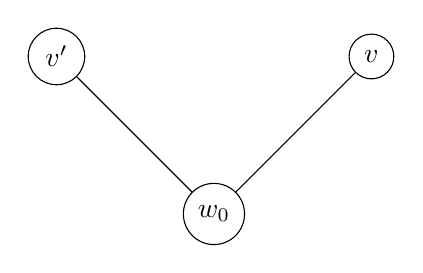
\begin{tikzpicture}[baseline={(0,0)}]
	\node[shape=circle,draw=black] (w) at (0,0) {$w_0$};
	\node[shape=circle,draw=black] (v) at (2,2) {$v$};
	\node[shape=circle,draw=black] (v') at (-2,2) {$v'$};
	\path [-] (w) edge node[left] {} (v);
	\path [-] (w) edge node[left] {} (v');
\end{tikzpicture}
\qquad
\qquad
\begin{tikzpicture}[baseline={(0,0)}]
	\node[shape=circle,draw=black] (w) at (0,0) {$w_0$};
	\node[shape=circle,draw=black] (w1) at (0,-2) {$w_1$};
	\node[shape=circle,draw=black] (wn) at (0,-4) {$w_n$};
	\node[shape=circle,draw=black] (v) at (2,2) {$v$};
	\node[shape=circle,draw=black] (v') at (-2,2) {$v'$};
	\path [-] (w) edge node[left] {} (v);
	\path [-] (w) edge node[left] {} (v');
	\path [-] (w) edge node[left] {} (w1);
	\path [dashed] (w1) edge node[left] {} (wn);
\end{tikzpicture}
\end{center}
\caption{The visualization of the models $\mathcal{K}$ (left) and
$\mathcal{K}^{(n)}$ (right)}
\end{figure}


It should be noted that for $w\in\mathcal{K}$ and for any formula $\gamma$
that we have:
$$\vDash_w\gamma\ \text{in}\ \mathcal{K}\Leftrightarrow\ \vDash_w^{(n)}\gamma\
\text{in}\ \mathcal{K}^{(n)}$$
For the rest of this project we will omit the annoying superscripts.

The following lemma will explain a bit deeper how these derived models works:

\begin{lem}
	\label{lem:GLS}
	Let $\mathcal{K}$ be a $\alpha$-sound model, $S(\alpha)$ the set of
	subformulas of $\alpha$ and $\mathcal{K}^{(n)}$ be the $n$-derived
	model. Then for all $\beta\in S(\alpha)$ we have:
	$$\vDash_{w_0}\beta\Leftrightarrow\vDash_{w_n}\beta$$
\end{lem}
\begin{proof}
	We will prove this by induction on $n$. The lemma will follow from the
	case $n=1$ [Why?], and this will be proven by induction om complexity
	of $\beta$. The only non trivial case is the case where
	$\beta=\Box\gamma$, so this is the only case that will be shown:

	Let $\beta=\Box\gamma\in S(\alpha)$. 

	\textbf{($\Rightarrow$)}\ The following is clear for
	$\Box\gamma\in S(\alpha)$:
	$$\vDash_{w_0}\Box\gamma\Rightarrow\vDash_{w_0}\gamma$$
	This follows since our model is $\alpha$-sound. Therefore we have:
	$\forall v>w_1(\vDash_{w_1}\gamma)$ and thus $\vDash_{w_1}\Box\gamma$

	\textbf{($\Leftarrow$)} Here we can make the following deduction:
	\begin{align*}
		\vDash_{w_1}\Box\gamma&\Rightarrow\forall
		v>w_1(\vDash_v\gamma)\\
				      &\Rightarrow\forall
				      v>w_0(\vDash_v\gamma)\\
				      &\Rightarrow\vDash_{w_0}\Box\gamma
	\end{align*}
\end{proof}
We can now return to our proof of the main theorem of this section by proving
\ref{thm:lll}
\begin{proof}[Proof of \ref{thm:lll}]
	We will start of by proving (1). One way is easy:

	\textbf{($\Leftarrow$)} If $\alpha$ is true in all $\alpha$-sound
	models $\mathcal{K}$ of $\GL$ then:
	$$\vdash_{\GL^s}\alpha$$
	And therefore we have $\vdash_\GLS\alpha$.

	\textbf{($\Rightarrow$)} This way takes a bit more work; it will be
	proven by contraposition. So suppose that $\alpha$ is false in
	$\alpha$-sound model $\mathcal{K}=\la W,R,\phi\ra$. Then we have:
	$$\vDash_w\bigwedge_{\Box\beta\in
	S_\Box(\alpha)}(\Box\beta\rightarrow\beta)$$
	But still also have: $\not\vDash_{w_0}\alpha$. We will show that
	$\not\vdash_\GLS\alpha$ by showing that for any finite set $\Gamma$
	that for the system
	$\GL^\Gamma=\GL+\bigwedge_{\gamma\in\Gamma}(\Box\gamma\rightarrow\gamma)$
	that we have:
	$$\not\vdash_{\GL^\Gamma}\alpha$$
	By lemma \ref{lem:GLS} we have that every  model in the sequence
	$\mathcal{K}^{(0)},\mathcal{K}^{(1)},\ldots$ is an $\alpha$-sound
	model, wherein $\alpha$ is false. We will just have to show that for
	any finite set $\Gamma$ that is a number $m$ such that:
	$$\vDash_{w_m}\bigwedge_{\gamma\in\Gamma}(\Box\gamma\rightarrow\gamma)$$
	This can be shown by showing that there is a $m$ such that for each
	$n>m$ that the following holds:
	$$\vDash_{w_n}\Box\gamma\rightarrow\gamma$$
	But we either have that $\vDash_{w_m}\Box\gamma$ for all $n$, thus
	$\vDash_{w_n}\gamma$ for all $n$; or we have
	$\not\vDash_{w_m}\Box\gamma$ for some $m$ and thus
	$\not\vDash_{w_n}\Box\gamma$ and
	$\vDash_{w_n}\Box\gamma\rightarrow\gamma$ for al $n>m$. This shows (1).
	We will now prove (2).

	The way "$\Rightarrow$" is trivial since if $\vdash_\GL\alpha$ then
	$\alpha$ is valid in all models of $\GL$\ and hence in all
	$\alpha$-sound models of \GL.
	
	For the implication $\Leftarrow$, we will assume that $\alpha$ is valid
	in all $\alpha$-sound models.  Again set $\GL^s$ to be
	$\GL+\bigwedge_{\Box\beta\in S_\Box}(\Box\beta\rightarrow\beta)$. Then
	we have that show that:
	\[\vdash_{\GL^s}\alpha\Rightarrow\ \vdash_\GL\alpha\]
	We show this by contraposition. So assume that $\vdash_\GL\neg\alpha$.
	We get $\GL^s$ be adding a finite amount of formulae to $\GL$\ and thus
	we have that $\vdash_{\GL^s}\neg\alpha$.
\end{proof}
In the chapter \ref{chap:Complete} it will be shown that \GL\ axiomatise the
provable schemata in \PRA\ and \GLS\ will axiomatise the \textit{true} schemata
of arithmetics; i.e truth in the standard model $\mathcal{N}=\la
\omega,+,\cdots\ra$ of arithmetics.
\end{document}
